% Chapter 6

\chapter{Example Problems}  % Main chapter title

\label{Chapter6}  % For referencing the chapter elsewhere, use \ref{Chapter1}

\lhead{Chapter 6. \emph{Example Problems}}  % This is for the header on each page - perhaps a shortened title

%----------------------------------------------------------------------------------------

The objective of IM3D code is to accurately and quickly calculate the 3D space-distributions of primary radiation damages in arbitrary-complex geometric targets containing different shapes and components, including electronic and nuclear energy depositions, back-scatted/implanted ions, $dpa$, interstitials, vacancies and sputtering atoms, etc. In the following, some verifications and examples are given to demonstrate the validity and capability of IM3D code.

\section{Verifications}

To verify the accuracy of IM3D code, three examples including the ion/damage depth-distributions in bulk/multi-layer targets are performed and compared with that of TRIM code and experiments. Furthermore, some confinements in using TRIM-like codes are discussed and clarified.

As shown in Fig.\ref{Fig.3}, the depth-distributions of ion deposition are calculated for Si bulk under Ar ion beam irradiation with different irradiation energies. A typical Gaussian-type profile of ion depth-distributions are obtained, which is in good agreement with that of TRIM code for all three ion energies, even for the absolute intensity values.

\begin{figure}[!ht]\centering
\includegraphics[width=1.0\textwidth]{fig3.pdf}
\caption{Comparison of IM3D results with TRIM predictions for Ar ion depth-distributions in Si bulk, under Ar ion
implantation with different energies of (a) $10~keV$, (b) $100~keV$ and (c) $1000~keV$ and normal incidence at the center point of the target.} \label{Fig.3}
\end{figure}

The vacancy depth-distributions for Ni bulk under He ion beam irradiation with different incident energies are given in Fig.\ref{Fig.4}. Again, good agreements between IM3D and TRIM codes are obtained for all three ion energies. The intensity ratios between the predictions of the FC and KP methods is around 2 as estimated by TRIM code\cite{Stoller:2013}. By comparing to the standard reference values estimated by MD and NRT model, Stoller et al. pointed out that there could be a fundamental problem in the SRIM model used to calculate the number of vacancies created\cite{Stoller:2013}. Borschel et al. also found an obvious discrepancy from Iradina code to TRIM code for the damage production within collision cascades\cite{Borschel:2011}. Since TRIM is not an open-source software, the certain fine details of its defect generation algorithms are not clearly described in both SRIM's manual and published papers\cite{Ziegler:2010}. Generally, this discrepancy should be due to the difference of the replacement fractions in the total displacement events which are determined only by a sharp cut-off threshold energy\cite{Borschel:2011}. This threshold energy is usually set as the displacement energy ($E_d$) as given in SRIM's manual and elsewhere\cite{Ziegler:2010,Borschel:2011}. While the replacement process should occur only when the energy of the trajectory atom after replacement is lower than the binding energy ($E_b$) in bulk. Otherwise, the trajectory atom after replacement will leave the lattice site and migrate to other position, which generate a pair of interstitial and vacancy. Thus, by using the binding energy $E_b$ instead of the displacement energy $E_d$ as the threshold of replacements, we directly reproduced the exact depth profiles with the same absolute values and also the same vacancy intensity ratio between the FC and KP methods. In addition, dynamic annealing process should occur at finite temperatures and the larger number of primary point defects at $0~K$ predicted by the FC method would finally decay to MD, KP or experimental values.
%Thus, it is no need to make much scene to the absolute primary damage concentration at $0~K$ because it is just a reference for practical irradiations at $T>0~K$.

\begin{figure}[!ht]\centering
\includegraphics[width=1.0\textwidth]{fig4.pdf}
\caption{Comparison of IM3D results with TRIM predictions for vacancy depth-distributions predicted by FC and KP methods in Ni bulk, under He ion irradiation with different energies of (a) $0.5~MeV$, (b) $1.0~MeV$ and (c) $5.0~MeV$ and normal incidence at the certer point of the target.} \label{Fig.4}
\end{figure}

People found that the range of defect depth-distributions calculated by SRIM package are usually shallower than that of experiments more or less, which generally attributed to an overestimation of the electronic stopping powers used in SRIM package (especially for low-energy heavy ions)\cite{Chang:2012,Zhang:2009,Paul:2013}. A reduced target density is simply employed to compensate for the overestimation of electronic stopping power and thus to reduce the discrepancy\cite{Chang:2012}. Through setting the target density lower, good agreements are obtained comparing to TRIM code and experimental results for $305~nm$ ZrO2 film on Si bulk under $2.0~MeV$ Au ion irradiation, as shown in Fig.\ref{Fig.5}. However, artificially changing of target densities is just a phenomenological treatment with no sound physical basis. Other influences should also be considered to understand this range discrepancy. When ion fluence is high enough, the defect depth-distributions would be physically changed by the evolution of the target density due to ion irradiation. While when ion fluence is not too high, the change of the target density in experiments can be neglected. Moreover, the profiles can further broaden into depth to approach to experiments when taking into account of the diffusion and reaction effects as discussed in our previous paper\cite{Li:2012}. Therefore, it is not only the change of target densities (or the electronic stopping powers) but most of all the diffusion and reaction effects cause the discrepancy, because the temperature in practice is finite other than $T=0~K$ set in TRIM-like codes. The diffusion and reaction effects become prominent especially for the case of ions with much high diffusivity in the target\cite{Li:2012}. These effects are non-equilibrium dynamic processes taking account of temperature and time, which should be described by the meso-scale simulation methods such as the kinetic Monte Carlo (KMC) and cluster dynamics (CD) models.

\begin{figure}[!ht]\centering
\includegraphics[width=0.6\textwidth]{fig5.pdf}
\caption{Comparison of IM3D results with TRIM predictions and SIMS measurement\cite{Chang:2012} for Au ion depth-distribution in $ZrO_2/Si$ sample, under Au ion irradiation with the energy of $2.0~MeV$ and normal incidence at the center point of the sample. IM3D and TRIM predictions under the assumption of the reduced density are also given, where $15\%$ reduced density for $ZrO_2$ ($4.6~g/cm^3$) and $27\%$reduced density for Si ($1.7~g/cm^3$) are used.} \label{Fig.5}
\end{figure}

%----------------------------------------------------------------------------------------
\section{Two effects: nano-size and geometric effects}

As the ion range or dimension of the collision cascades becomes comparable to the size of the nanoobject itself, the high surface-volume ratio of nanostructured materials will induce two new effects, i.e., the so-called nano-size effect and geometric effect.

Due to the surface reconstruction of nanostructure materials, the thermodynamic properties change with the size reduction, which cause the nano-size effect. In Fig.\ref{Fig.6}(a), the amount of defects along with irradiation energies calculated by IM3D code has the similar trend to that of the analytical model and MD simulation (with the maximum amount produced at energies around $3~keV$), while is smaller than that of MD simulations. This discrepancy should come from the nano-size effects like the difference of stopping powers and the decrease of energy thresholds (i.e., the displacement and binding energies) between nanostrucutres and bulk, etc. While these energy thresholds are usually lower with the size reduction of nanostructures and follow a universal relation as predicted for the cohesive energy of nanoparticles as in Ref.\cite{Vanithakumari:2008}. It would underestimate the total number of defects for both $3$ and $4-nm$ nanowires if the bulk energy thresholds are used for determining the capability of defect generation. This viewpoint can just be proved by using the half values of bulk energy thresholds to decrease the discrepancy between IM3D and MD simulations for the $3-nm$ nanowire. The interstitials, vacancies and sputtering atoms are directly relate to the energy thresholds (especially the surface/lattice binding energies), which are influenced by the nano-size effect mostly. The discrepancy between IM3D and MD simulations thus becomes more obvious when irradiation energy is larger (see Fig.\ref{Fig.6}(b)).

In IM3D code, we consider the bulk parameters are valid at least when the target size is larger than $\sim 10~nm$, because in this case the thermodynamic properties close to constants and the nano-size effect is vanishing\cite{Ouyang:2008}. For the target size smaller than $\sim 10~nm$, IM3D code can also be employed to estimate the primary radiation damages at the first approximation by using a set of modified parameters considered the nano-size effects, while MD method would prefer to be used to give a more accurate estimation because of the acceptable calculation consuming. Furthermore, Fig.\ref{Fig.6} (b) shows that both the nano-size and geometric effects determine the number of defects, that is, the amount of different types of defects for the flat case is higher than that of edge due to the geometric effect. The difference between the flat and edge cases is smaller than that of MD results\cite{Ren:2012}, because no channeling effect is included in IM3D code for an amorphous target.

\begin{figure}[!ht]\centering
\includegraphics[width=0.49\textwidth]{fig6-a.pdf}
%\label{Fig.1a}
\includegraphics[width=0.46\textwidth]{fig6-b.pdf}
%\label{Fig.1b}
\caption{(a) Comparison of the number of vacancies in GaN nanowire along with Ar ion energies predicted by IM3D code, the analytical model based on TRIM code and MD simulations. The curves for the analytical model are artificially scaled to have the same area as the ones obtained from MD simulations, for the absolute amount of damage cannot be estimated reliably from the results based on SRIM calculations\cite{Ren:2012}. IM3D-1 and IM3D-2 are corresponding to the bulk energy thresholds and half values of the bulk thresholds used in the simulations, respectively. (b) The respect and total numbers for three different types of defects (vacancies, interstitials and sputtered atoms) along with Ar ion energies, for the 3 and $4~nm$-diameter GaN nanowire under Ar ion irradiation at the edge and facet of GaN nanowire.} \label{Fig.6}
\end{figure}

The geometric effect will influence the trajectory of an ion when it transport through the interface between two different material zones, such as trajectory emission, re-entering, sputtering and shading, etc. In order to illustrate the geometric effect contrast to the bulk counterpart, we simulate the vacancy depth-distributions in Au column target under two types of ion beams (i.e. center and random incidence), as shown in Fig.\ref{Fig.7}. The ranges of vacancy depth-distributions and the total amount of vacancies are both increase with the increasing of column diameters, and finally approach to the bulk values after the critical diameters (around $200~nm$ and $1000~nm$ for center and random ion incidence, respectively).

Assumes that the radial distribution of damages (e.g. vacancies) $I \left( r \right)$ produced by an ion in a half-infinite bulk target follows a exponential decay (as shown by the inserted figure in Fig.\ref{Fig.7}(a)),

\noindent
\begin{equation}
I\left(r\right) = I_0 e^{-r/t},~~r \in \left[0, \infty\right), \label{Eq.1}
\end{equation}

\noindent where, $I_0$ is the intensity of damages at $r=0$ and $t$ is the effective attenuation length of damages in radial direction ($25~nm$ for center ion incidence). The amount of damages in a nanowire for the center ion beam incidence can be obtained by integrating Eq.(\ref{Eq.1}) over the volume of the antisymmetric column (see Fig.\ref{Fig.7}) that,

\begin{equation}
N_d = \int_{0}^{R} \int_{0}^{2\pi} I\left(r\right)drd\theta = \frac{2 \pi I_0}{t} \left(1-e^{-R/t}\right), \label{Eq.2}
\end{equation}

\noindent where R is the radius of the column.

Similarly, we can give the analytical function for the random ion beam incidence, by additionally considering the effective attenuation range $t$ ($32~nm$ for random ion incidence) of the spread ion beam. For $R \leq t$, we assumed that the amount of damages also follows Eq.(\ref{Eq.2}) approximately but with $t=32~nm$ instead. While for $R > t$, only ions bombarding in the effective attenuation range $t$ from the colume side with the area ratio of $\left( \frac{2t}{R} - \frac{t^2}{R^2} \right)$, can cause a half loss of defects with the ratio of $0.5 \cdot \left(1 - \frac{1}{e}\right)$ as estimated approximately from Eq.(\ref{Eq.2}) with $R = t$. Otherwise, no loss of the defects when ions bombarding in the central zone $(0,~R-t)$ of the column. Thus, the amount of damages follows that,

\begin{equation}
N_d = \frac{2 \pi I_0}{t} \left[1 - 0.5 \cdot \left( \frac{2t}{R} - \frac{t^2}{R^2} \right) \left(1 - \frac{1}{e}\right) \right],~ R > t. \label{Eq.3}
\end{equation}

\noindent It can be found as shown in Fig.\ref{Fig.7} that these two simple analytical estimations can fit the calculated vacancy-diameter relation much well, which directly illustrates that the geometric effect is the main factor to the distributions of primary radiation damages in nanostructured materials.

\begin{figure}[!ht]\centering
\includegraphics[width=0.49\textwidth]{fig7-a.pdf}
%\label{Fig.1a}
\includegraphics[width=0.49\textwidth]{fig7-b.pdf}
%\label{Fig.1b}
\caption{The depth-distributions and the total number of vacancies for Au nanowaire with different diameters under $45~keV$ Ne ion irradiation with the (a) center and (b) random normal-incidence beams. Eqs.(\ref{Eq.2}) and (\ref{Eq.3}) are plotted to fit the relations of the total number of vacancies with different diameters. The inserted figures in (a) and (b) show the vacancy radial-distribution in Au bulk and the vacancy space-distribution in Au nanowire with the diameter of $120~nm$, respectively.} \label{Fig.7}
\end{figure}

Column is a typical model of a class of nanostructured materials, such as nanowire, nanoporous and ``fuzz''. Bringa et al. performed a serial of experimental studies on the anti-irradiation behaviors of nanoporous materials and proposed an anti-irradiation window by simply considering of the effective vacancy diffusivity and lower critical size due to melting. However, they did not consider the contribution from the change of primary radiation damages by the geometric effect and just assumed that the primary radiation damages is a constant value. As shown here, the geometric effect can introduce a dramatical reduction of the primary radiation damages, which should be taken into account in the estimation of the anti-irradiation window. Furthermore, by considering the primary damage distributions as well as the diffusion and reaction effects at $T > 0~K$, CD model would be performed to give the more accurate anti-irradiation windows of nanostructure materials in the future.

%----------------------------------------------------------------------------------------
\section{Applications}

\subsection{Arbitrary complex targets based on CSG and FETM methods}

To our knowledge, IM3D is the most universal and robust code for simulating of the primary radiation damages in arbitrary complex targets with different shapes and components till now. Based on CSG geometric model, nine basic shapes (in Fig.\ref{Fig.8}(a)) and their assemblies (in Fig.\ref{Fig.8}(b)) can be constructed at present to model many regular targets with different materials. The geometric effect makes the distinctions of the defect space-distributions among different shapes.

\begin{figure}[!ht]\centering
\includegraphics[width=0.32\textwidth]{fig8-a.pdf}
%\label{Fig.1a}
\includegraphics[width=0.21\textwidth]{fig8-b.pdf}
%\label{Fig.1b}
\includegraphics[width=0.44\textwidth]{fig8-c.pdf}
%\label{Fig.1b}
\caption{(a) $Dpa$ space-distributions of nine basic shapes based on CSG geometric method and composed of Si under $10~keV$ He ion irradiation with the random normal-incidence beam. (b) $Dpa$ space-distribution of for a 100 nm-diameter Cu/Fe nano-bicrystal constructed by CSG geometric method under $200~keV$ He ion irradiation with the random normal-incidence beam. The insert scatter line is the corresponding He ion depth-distribution. (c) The respect and total He ion depth-distributions for different energies He ions (left) and the $dpa$ (right) space-distribution for $100~keV$ He ions with the random normal-incidence beam irradiated on a $130~nm$ NiP metallic glass nanostructure constructed by FETM geometric method.} \label{Fig.8}
\end{figure}

By introducing the geometric effect, more reliable information can be obtained when estimate the defect (such as ion and $dpa$) distributions. For bulk/multi-layer systems, people usually employ TRIM code to give the first approximation of ion/dpa distributions. However, for complex nanostructures as mentioned in Refs.\cite{Liontas:2014,Landau:2014}, errors would be introduced when using TRIM code. As shown in Fig.\ref{Fig.8}(b), more practical $dpa$ space-distribution is obtained for a Cu/Fe nano-bicrystal based on CSG geometric model. For NiP metallic glass nanostructures (in Fig.\ref{Fig.8}(c)), more accurate ratio of ion fluence can be estimated to generate a uniform distribution damage based on FETM geometric model, with $1:3.2:4:8$ instead of $3.5:4.0:2.8:5.5$ in Ref.\cite{Liontas:2014}. Thus, the geometric effect can dramatically change the behaviors of ion irradiation and can not be neglected.

\subsection{Nano-yttria in ODS steels under ion-irradiation}

Recently, ODS steels (with a great mount of yttria ($Y_2O_3$) nanopartiles embedded in a steel matrix) have been termed as a new class of high anti-irradiation and high strength nanostructured nuclear materials\cite{Chen:2013,Brimbal:2014,Fave:2014,Huang:2014,Lazauskas:2013,Lescoat:2012}. However, the high radiation resistant mechanisms and the role of the embedded nanoparticles are still unclear and sometimes controversial. Moreover, the impact of primary damage processes on their high radiation resistant properties should also be discussed in detail. Here, we assumes a perfect iron matrix in which $Y_2O_3$ nanoparticles are embedded as a simplified model of an ODS steel and simulate the space-distributions of the primary radiation damages with the displacement energies of $40~eV$\cite{Ziegler:2010} for Fe and $57~eV$ for Y and O\cite{Lescoat:2012}.

\begin{figure}[!ht]\centering
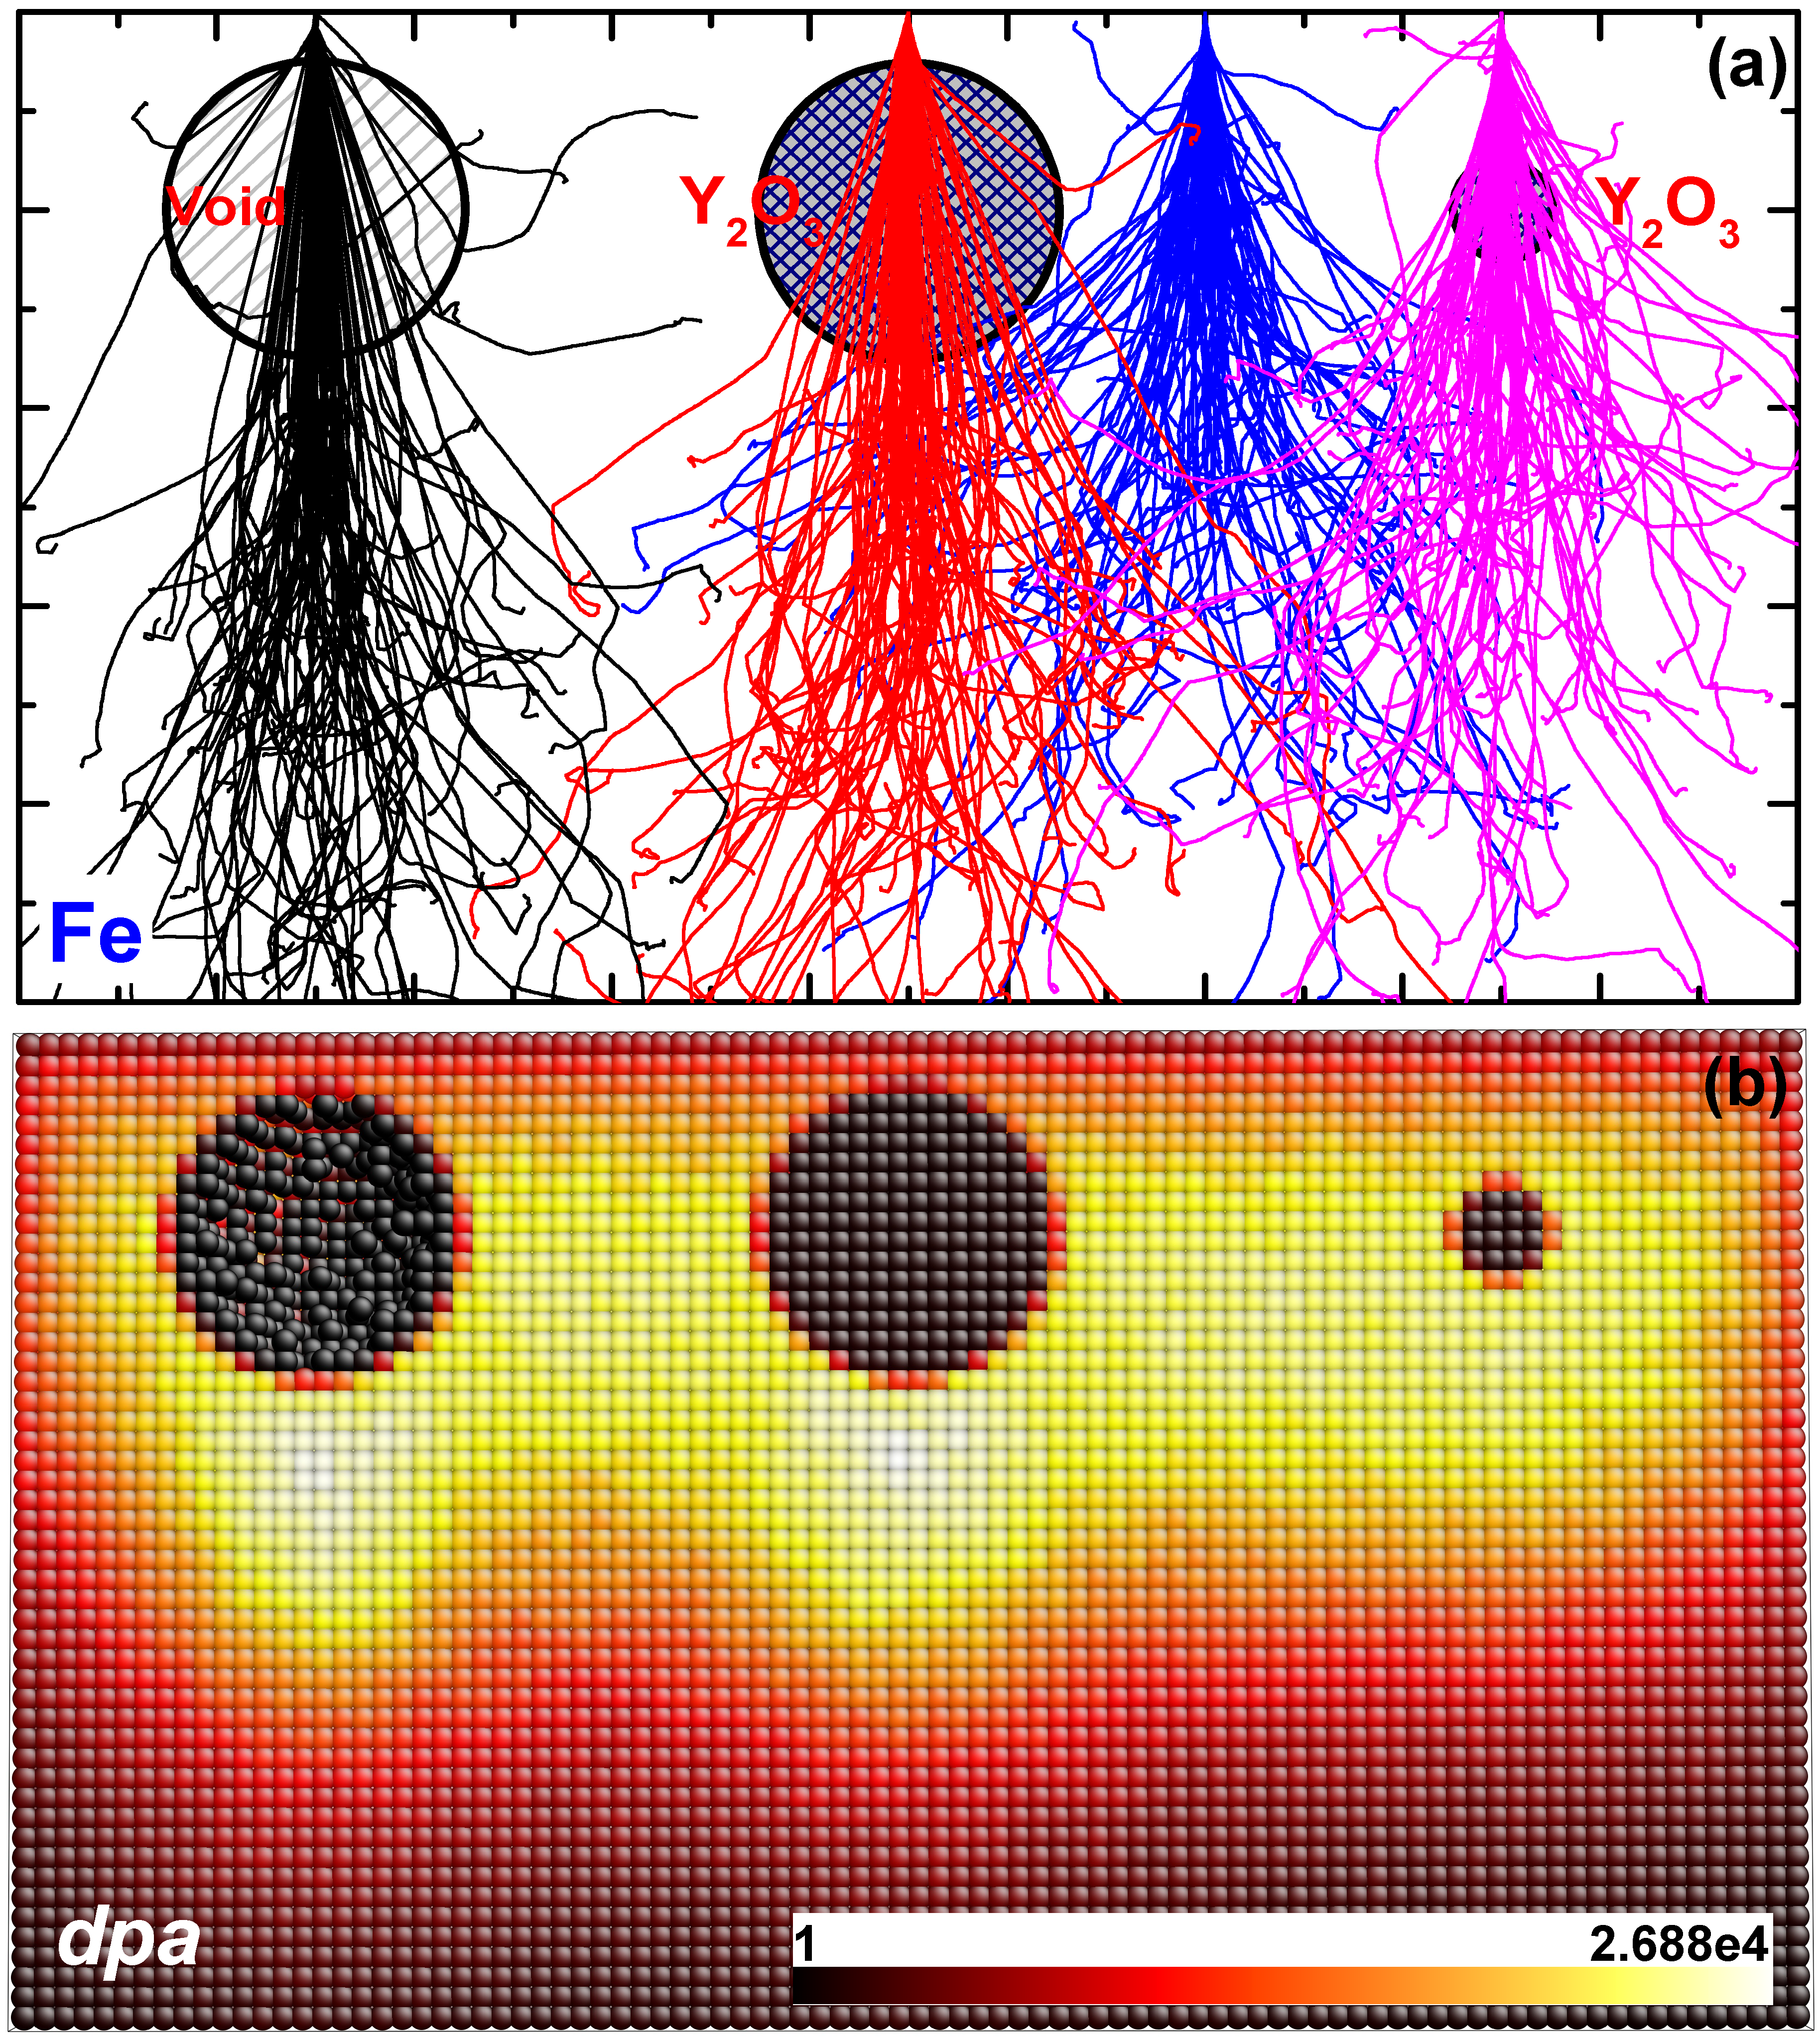
\includegraphics[width=0.5\textwidth]{fig9.pdf}
\caption{The (a) ion trajectories and (b) $dpa$ distribution cross-section for a target of Fe matrix with a void ($30~nm$) and two $Y_2O_3$ nanoparticles ($30~nm$ and $10~nm$) of different sizes embedded under $150~keV$ Fe ion irradiation with the random normal-incidence beam.} \label{Fig.9}
\end{figure}

Based on IM3D code, the ion trajectories and 3D space-distributions in a target of Fe matrix with a void and two $Y_2O_3$ nanoparticles of different sizes embedded can be given as shown in Fig.\ref{Fig.9}. Spheres with different materials/vacuum can change ion trajectories (Fig.\ref{Fig.9}(a)) by influencing the energy losses and the production rate of defects, and finally induce the different damage distributions (in Fig.\ref{Fig.9}(b)). Comparing to bulk regions, ions in void transport straightly without energy loss and penetrate into depths to generate more damages in the deep (i.e., the enhancement effect, similar to the MD results\ref{Lazauskas:2013}). Similarly, ions can also loss less energy and generate less damages in $Y_2O_3$ nanoparticles. Thus, $Y_2O_3$ nanoparticles are play the same role as voids to suppress the production of primary radiation damages but without losing the strength of the steel. The anti-irradiation of $Y_2O_3$ nanoparticles is mainly due to the lower defect generation rate with their much lower atomic density ($1.10934 \times 10^{22}~atoms~cm^{-3}$) comparing to that of the steel matrix ($8.388 \times 10^{22}~atoms~cm^{-3}$), the higher displacement energies of Y and O ($57~eV$) to that of Fe ($40~eV$), as well as the attraction of defects to the nanoparticle interface during annealing. The enhancement effect of $dpa$ intensity behind the void and  the bigger-size $Y_2O_3$ nanoparticle comes from the overlapping of the $dpa$ generated by the penetrating ion though the void / nano-particle and the ion directly transporting in iron matrix nearby, as shown in Fig.\ref{Fig.9}(a). This enhancement effect would induce a little more serious primary damages to Fe bulk matrix, which introduce a negative effect on the radiation resistant. While the enhancement effect can be reduced/removed by decreasing the diameter of $Y_2O_3$ nanoparticles from $30~nm$ to $10~nm$ as shown in Fig.\ref{Fig.9}(b), which has also been proved by the high resolution TEM measurements\cite{Lescoat:2012}. The high sink strength of the interface between $Y_2O_3$ nanoparticles and Fe matrix would also neutralize the enhancement effect and finally reduce the total damages in ODS steel after annealing.

\subsection{Ion beam sputtering induced the bending of W nanowire}

Under ion beam irradiation with high fluence, nanowires have been observed to bend towards and finally align with the ion beam\cite{Cui:2013}. The primary radiation damages should play an important role on this effect, which can also be studied by IM3D code feasibly. By generating a target with 3D surface mesh with FETM geometric method beforehand (in Fig.\ref{Fig.10}(a)) and inputting it into IM3D code, the 3D distribution of defects can be given such as vacancies for a bended W nanowire under the irradiation of Ga ion with the incident direction of 40 degrees and the energy of $150~keV$, as shown in Fig.\ref{Fig.10}(b). More primary vacancies generated on the side towards to the ion beam, making the density on this side lower than the other side and thus bend the column line. During the ion irradiation of W nanowire at finite temperatures, most of interstitials with a low migration energy ($0.013~eV$\cite{Derlet:2007}) would anneal with vacancies immediately, diffuse to the other side or deposit directly. While a little part of vacancies without annealing by interstitials are nearly immobile and stay constant with a much higher migration energy ($1.66~eV$\cite{Becquart:2007}). Here, in order to consider the final remaining damages in W nanowire, we use the difference value of vacancies minus interstitials by assuming annihilation of defects only occur in each cell ($10 \times 10 \times 10~nm^3$). An inhomogeneous distribution of the remaining defects is given in Fig.\ref{Fig.10}(c), where excess vacancies remain on the side towards to the ion beam and excess interstitials remain at the opposite side. Thus, a bending momentum (under inner stress due to an inhomogeneous expansion of the nanowire) towards the ion beam is induced to compensate the density difference until the the direction of the column line along the direction of ion beam, as observed in the experiment\cite{Cui:2013}. Moreover, the shading/shadowing effect (shading of the ions on their incident path by a particle leads to a decrease of damages behind the particle) can also be seen in Fig.\ref{Fig.10}(b) with dark area in the substrate appear behind the nanowire. During the plasma-surface interaction (PSI) process in PFMs (as shown below), these two typical effects (i.e., the bending and shading effects) should also occur at the reconstructed surface, causing the formation of complex ``fuzz'' nanostructure finally.

\begin{figure}[!ht]\centering
\includegraphics[width=1.0\textwidth]{fig10.pdf}
\caption{The (a) 3D surface mesh with FETM geometric method, (b) vacancy space-distribution and (c) remaining excess vacancies for a bended W nanowire under randomly distributed Ga ion sputtering with the incident direction of 40 degrees and the energy of $150~keV$.} \label{Fig.10}
\end{figure}

\subsection{D retention in W with roughness surface}

Plasma-surface interaction (PSI) is one of the most important issue in nuclear fusion instruments. Under low energy (in the range of $10 - 100~eV$), high flux (up to the order of $10^{24}~m^{-2}s^{-1}$) D/T/He plasma loads in ITER\cite{Wirth:2014}, the near surface morphology of PFMs will be dramatically changed and reconstructed to roughness or even more complex nanostructures like ``fuzz". These roughness nanostrucutes would further increase the retention of D/T/He. While T retention is also another key problem need to be widely studied. Thus, the calculation of the primary retention of H isotopes in W with roughness structures is much helpful for the understanding of the mechanisms of surface damage and T retention in PFMs.

In Fig.\ref{Fig.11}, we performed the W bulk with different rough-surface under D ion irradiation. A simple geometric model based on FETM method are used here to simulate the roughness structures\cite{Li:2008}. The rough-surface is constructed in a finite element triangulated mesh by using a Gaussian function to describe the distribution of the amplitude ($3 \sigma$) of the random roughness peaks as well as a uniform square mesh with a lattice constant ($a = 50 ~nm$) to describe the density of the roughness peaks. The depth-distributions of D in W are given for different rough amplitudes ($3 \sigma$) from $9$ to $1000~nm$ (in Fig.\ref{Fig.11}(b)). We found that the range of D ions in W increase with the increasing of rough amplitude. The distributions relate to Gaussian distribution directly, which can be approximated by the convolution of the effective interaction range and the geometric distribution of rough-surface, as shown in Fig.\ref{Fig.11}(b). Also, the geometric and shading effects dominate the behavior of D retention in W bulk with roughness surface.

The relation of D retention rate with the rough amplitude is also given in Fig.\ref{Fig.11}(c). With the increasing of the rough amplitude, D retention rate decreases at first and then increase after a critical point at about $3 \sigma = 50~nm$. It should be due to the competition of the enhancements of both the backscattering at glancing incidence and the shading effect by rough peaks. In order to describe the exact relation of the retention rate with the geometric and shading effects, a simple model is introduced to fit this relation. For the amplitude and distance of the roughness peaks are set as $3 \sigma$ and $a$, the effective incident angle of ions related to rough-surface is $\alpha \doteq arccos \left( \frac{a}{\sqrt{\left(3 \sigma \right)^2 + \left( a \right)^2}} \right)$. The backscattering coefficient $\eta \left(\alpha \right)$ is the function of this effective incident angle $\alpha$, which can be calculated by IM3D code directly. Thus, for the zero-order approximation, the primary retention rate of ions is equal to,

\noindent
\begin{equation}
R_0 \left( \alpha \right) \doteq 1 - \eta \left(\alpha \right), ~~all~3 \sigma. \label{Eq.4}
\end{equation}

\noindent Here, we assumed that it is actually true when $3 \sigma \leq z_0$, where $z_0 = 50~nm$ is used. While for $3 \sigma > z_0$, a fraction of backscattered ions would be shaded and redeposited by the roughness peaks, the shading probability can be estimated by the geometric effect as $P_s = \int_{0}^{\alpha} sin \left( \theta \right) d \theta = 1 - cos \alpha$. Thus, by assuming that all of the shaded ion are redeposited by the roughness peaks for the first-order approximation, the primary retention rate of ions can be described by,

\noindent
\begin{equation}
R_1 \left( \alpha \right) \doteq \left( 1 - \eta \left( \alpha \right) \right) + \eta \left( \alpha \right) \left( 1 - cos \alpha \right) = 1 - \eta \left( \alpha \right) cos \alpha, ~~ 3 \sigma > z_0. \label{Eq.5}
\end{equation}

\noindent If considering there is still some probability ($R_1$ is approximately used here) for the escaping of the shaded ions by roughness peaks, a more accurate estimation of the primary retention rate of ions in rough-surface can be given by a second-order approximation base on the predictor-corrector method,

\noindent
\begin{eqnarray}
& R_2 \left( \alpha \right) & \doteq \left( 1 - \eta \left( \alpha \right) \right) + R_1 \left( \alpha \right) \eta \left( \alpha \right) \left( 1 - cos \alpha \right) \nonumber \\
&&{} = 1 - \eta \left( \alpha \right) cos \alpha - \eta ^2 \left( \alpha \right) cos \alpha + \eta^2 \left( \alpha \right) cos^2 \alpha, ~~ 3 \sigma > z_0. \label{Eq.6}
\end{eqnarray}

\begin{figure}[!ht]\centering
\includegraphics[width=0.65\textwidth]{fig11-a.pdf}
%\label{Fig.1a}
\includegraphics[width=0.51\textwidth]{fig11-b.pdf}
%\label{Fig.1b}
\includegraphics[width=0.47\textwidth]{fig11-c.pdf}
%\label{Fig.1c}
\caption{(a) The D ion space-distribution for W roughness surface with the roughness amplitude of $3 \sigma = 60~nm$ and the roughness constant of $a = 50~nm$. (b) The D ion depth-distributions and the fitting profiles by Gaussian functions for W roughness surface with different roughness amplitudes ($3 \sigma$) and the roughness constant of $a = 50~nm$. (c) The D retention ratio and the fitting Eqs.(\ref{Eq.4}) and (\ref{Eq.6}) along with the roughness amplitudes for W roughness surface with the roughness constant of $50~nm$. Here, all W roughness surfaces are under the irradiation of $100~eV$ D ion beam with the random normal-incidence.} \label{Fig.11}
\end{figure}

A good agreement can be given based on the rough estimations by Eq.(\ref{Eq.4}) for $3 \sigma \leq z_0$ and Eq.(\ref{Eq.6}) for $3 \sigma > z_0$ (as shown in Fig.\ref{Fig.11}(c)), which demonstrates that the geometric and shading effects are the main contributions to the enhancement of the primary D retention in W. At finite temperature or especially high temperatures (typically $400 - 800~^\circ C$ in ITER\cite{Wirth:2014}) in fusion instruments, interstitial D atoms will diffusion quickly, most of which would desorb from surface. While, if the influence of the diffusion effect is fixed, the primary retention rate would be the only key factor to the D retention, especially when the surface of PFMs becomes roughness. Furthermore, the retention of D/T/He in ``fuzz" structures should also follow the same trend at a first glance.
